% !TEX TS-program = xelatex
% !TEX encoding = UTF-8 Unicode
% !Mode:: "TeX:UTF-8"
% !TeX root = resume.tex
\documentclass{resume}
\usepackage{styles/zh_CN-Adobefonts_external}
\usepackage{styles/linespacing_fix}
\usepackage{cite}
\usepackage{graphicx} % 用于插入图片
\usepackage{array}    % 用于 m{} 列类型和 @{} 来去除列间距

% 压缩竖直间距以适配单页（不改变字号）
\usepackage{geometry}
\geometry{a4paper, left=0.75in, right=0.75in, top=0.4in, bottom=0.35in, nohead}
\titleformat{\section}{\Large\bfseries\raggedright}{}{0em}{}[\titlerule]
\titlespacing*{\section}{0cm}{*0.25}{*0.35}
\setlist[itemize]{topsep=0.05em, itemsep=0.02em, parsep=0pt, leftmargin=1.5pc}
\linespread{0.98}

\begin{document}
\pagenumbering{gobble} % 吞掉页码
\vspace{-5pt}
\noindent

% 右上角证件照（零高度叠加，不影响居中姓名/联系方式）
\raisebox{-1.7cm}[0pt][0pt]{\makebox[\textwidth][r]{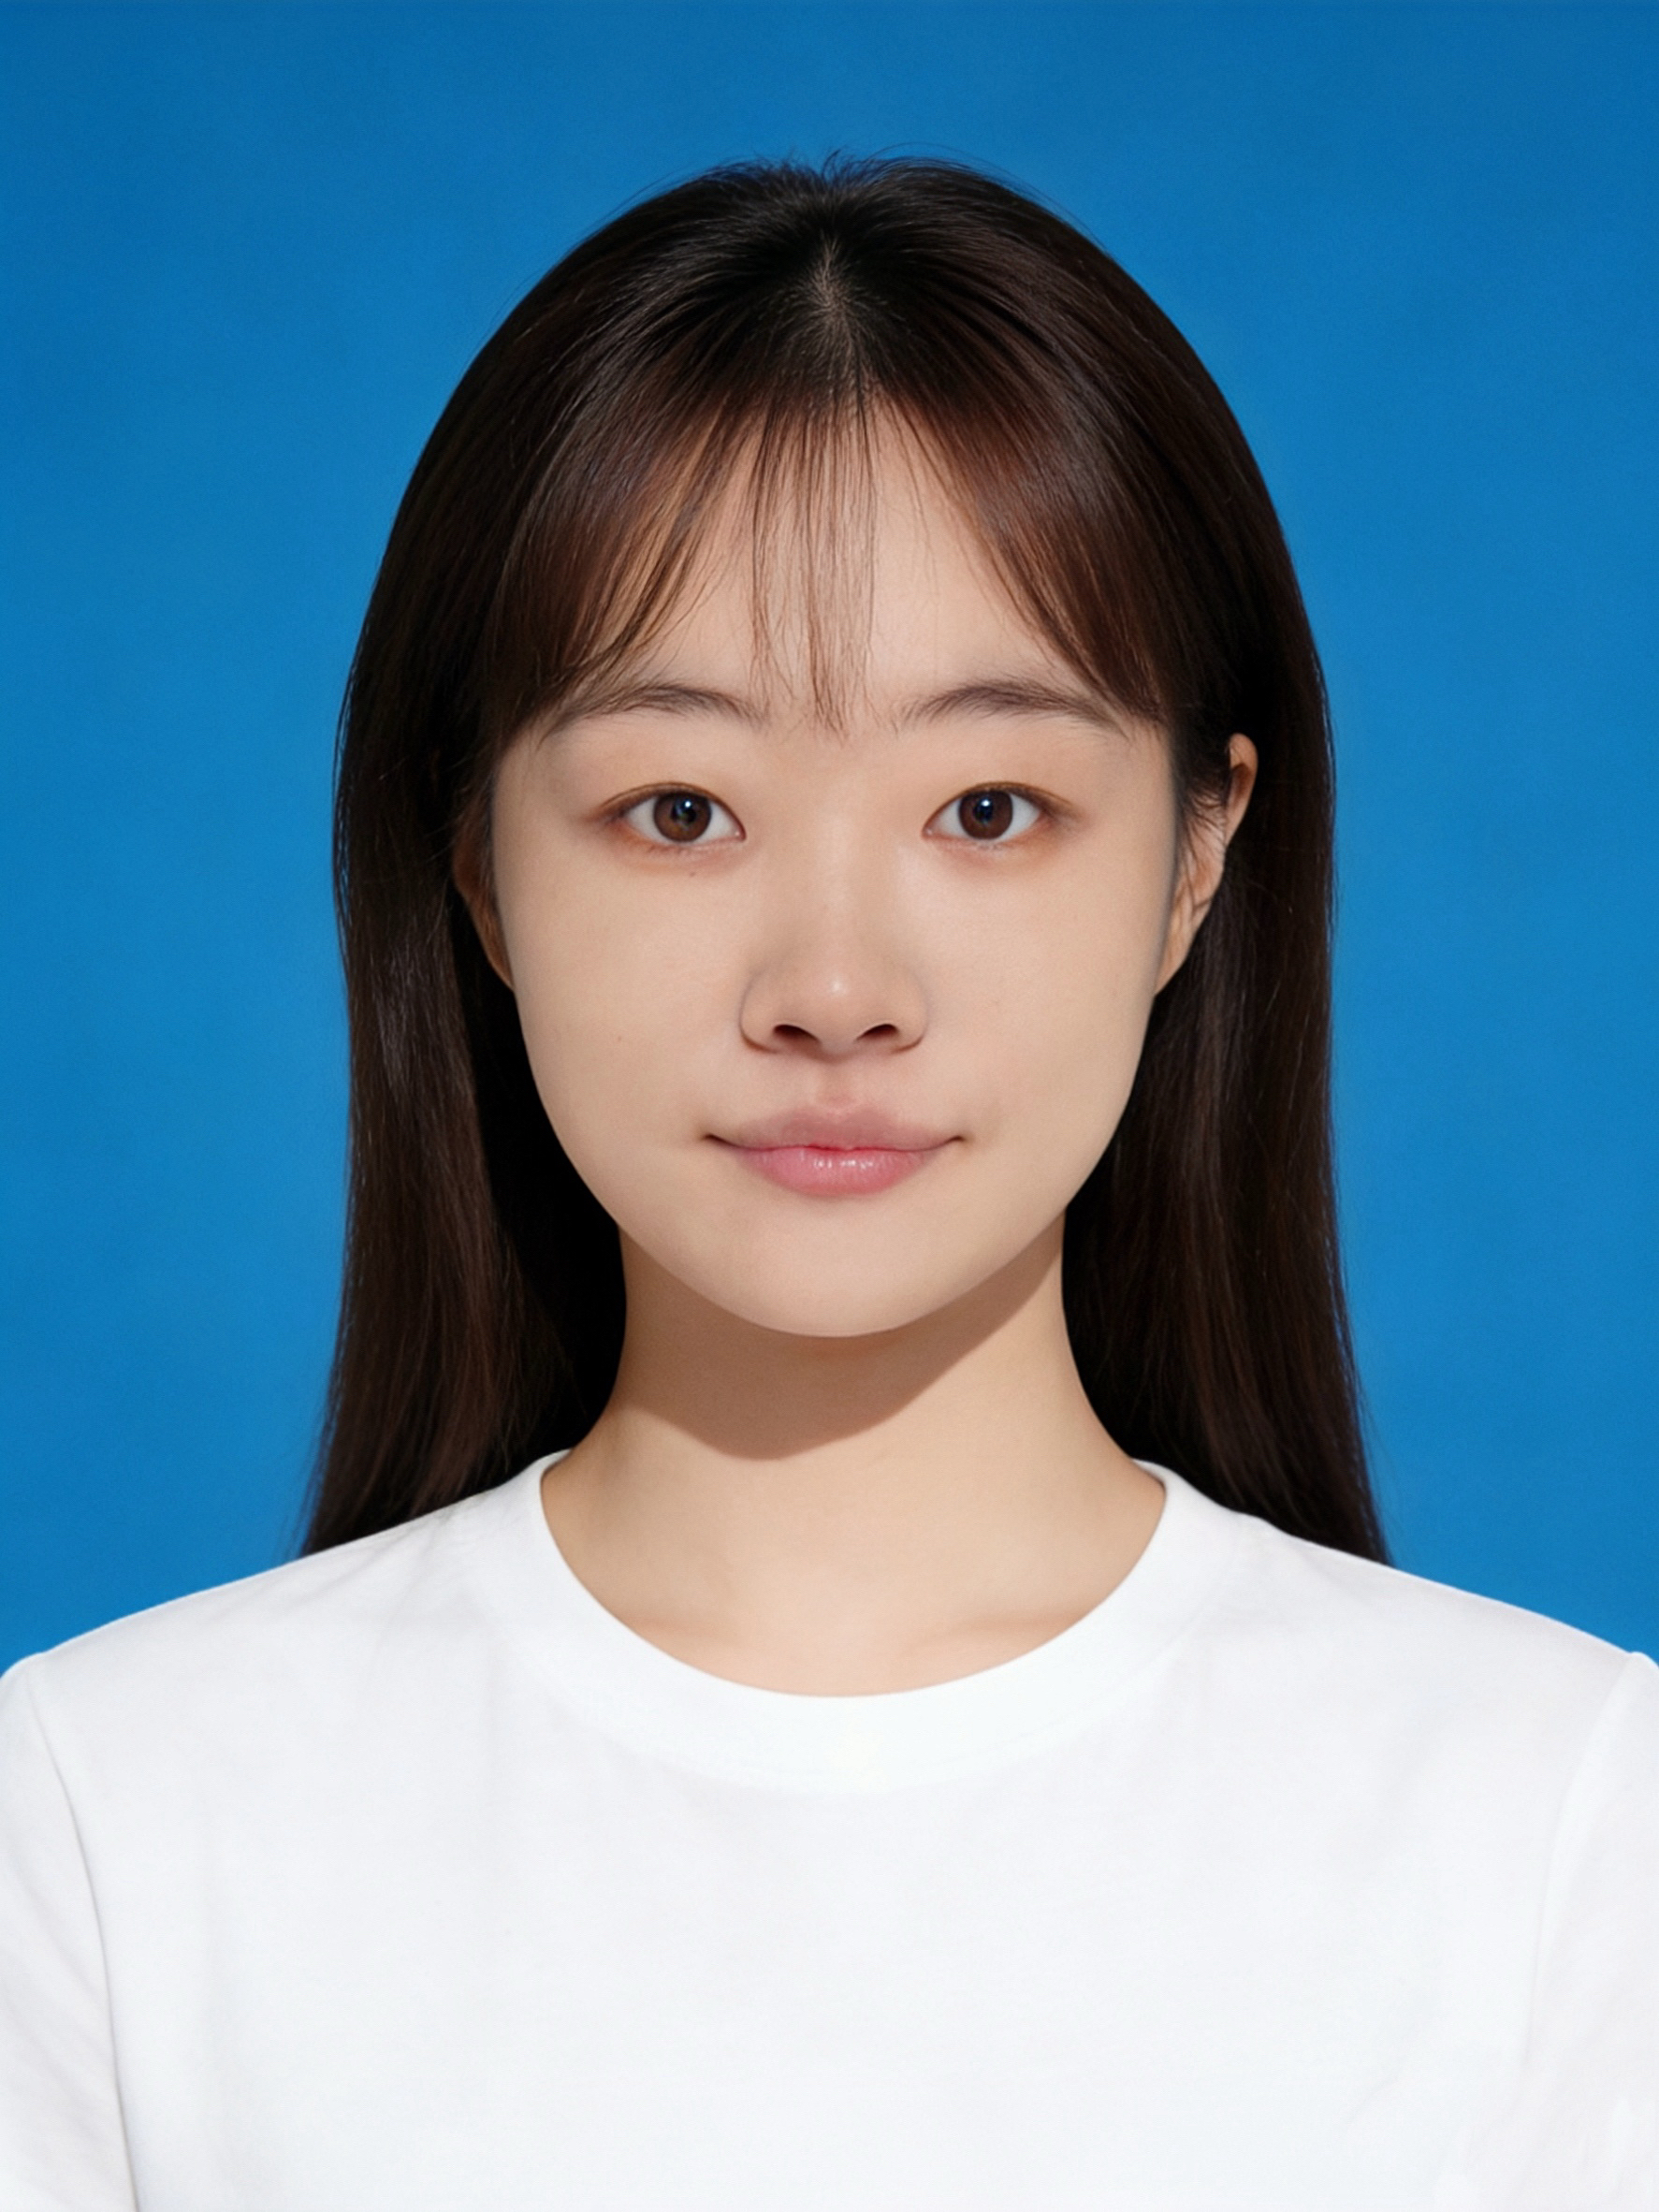
\includegraphics[height=2.8cm,keepaspectratio]{./imgs/photo.jpg}}}%
\name{陈可}
\basicInfo{
\phone {\textbf{(+86) 15174759971}} /\
\emaillink{chenke9971@gmail.com}{\textbf{chenke9971@gmail.com}}
}

\section{\ 教育背景}
\noindent
\makebox[0.3\textwidth][l]{\textbf{吉林大学--硕士(推免)}}%
\hfill
\makebox[0.4\textwidth][c]{\textbf{软件学院/软件工程}}%
\hfill
\makebox[0.3\textwidth][r]{2024.06 -- 至今}\par
\noindent
\makebox[0.3\textwidth][l]{\textbf{吉林大学--本科}}%
\hfill
\makebox[0.4\textwidth][c]{\textbf{软件学院/数据科学与大数据技术}}%
\hfill
\makebox[0.3\textwidth][r]{2020.09 -- 2024.06}\par

\section{\ 实习经历}
\noindent
% TODO: 占位内容（照搬自 ljc 模板），之后替换为陈可本人的实习经历
\makebox[0.3\textwidth][l]{\raisebox{-0.8ex}{
\includegraphics[width=0.028\textwidth]{./imgs/jd_logo.png}}~\textbf{京东-京东零售-广告智能部}}%
\hfill
\makebox[0.4\textwidth][c]{\textbf{算法实习生}}%
\hfill
\makebox[0.3\textwidth][r]{\normalsize 2026.05 -- 至今}\par
\vspace{0.3ex}
\textbf{基于 LLM 反事实先验的广告主激励因果建模}： 在有限广告激励资源下，核心是识别“因激励才会采纳”的高增量广告主；建模为因果推断任务，重点应对反事实不可观测、采纳正样本稀疏及激励非随机下发导致的强混杂问题。
\begin{itemize}
  % \item \textbf{问题:} 在有限广告激励资源下，核心是识别“因激励才会采纳”的高增量广告主；建模为因果推断任务，重点应对反事实不可观测、采纳正样本稀疏及激励非随机下发导致的强混杂问题。
  \item \textbf{贡献：} 利用 Transformer 统一建模序列与非序列异构特征，通过显式 Uplift Head 直接预测个体激励增量；引入 \textbf{LLM 双情境反事实推理补充稠密增量监督}，并利用 Doubly Robust 正交排序融合真实反馈。
  \item \textbf{结果：} 在 60 万条业务数据上，测试集 AUUC 相对最强基线提升 \textbf{67.5\%}；\textbf{形成一篇论文在投}。
\end{itemize}
\vspace{0.3ex}
\textbf{基于 LLM 商品理解的广告 ROI 预测与投前建议}：针对商品类目挂载偏差及\textbf{冷启动商品}历史投放信息不足导致的 ROI 建议不准问题，从商品内容出发，建模为融合语义与业务属性的 ROI 预测。
\begin{itemize}
  \item \textbf{贡献：} 基于 Qwen3-Embedding-8B 构建相似商品召回与 ROI 预测框架；针对“文本相似但 ROI 表现差异大”的问题，设计 Hard Negative 三元组微调，将商品表征由通用语义空间对齐至 ROI 表现空间，提升预测准确性。
  \item \textbf{结果：} 在 422 万条业务数据上构造 18.8 万条训练三元组，Top10\% 高 ROI 商品命中率由 68.6\% 提升至 74.9\%，支撑冷启动商品的投前 ROI 建议。
\end{itemize}

\section{\ 项目经历}
\noindent
\textbf{自研 Agent 可靠性增强与分层工作记忆系统}\par
\datedline{\textit{核心开发者}}{2026}
\begin{itemize}
  \item 面向多步骤工具任务中 Agent 输出不稳定、长上下文冗余影响后续决策的问题，从零搭建类 Agent 执行框架，完成\textbf{任务解析、上下文组织、工具编排、结果生成与状态返回}等核心模块设计
  \item 设计 \textbf{Result Evaluator} 对最终结果进行任务完成度、格式合法性与证据完整性校验
  \item 设计\textbf{分层工作记忆机制}，将记忆组织为摘要层、结构化状态层和详细证据层；基于 task-oriented compact 对用户偏好、工具调用结果、可复用流程等进行压缩更新，以 working memory 替代全历史上下文参与后续执行
  \item 在多步骤任务上，相比 baseline 实现\textbf{任务成功率提升 12\%、一次通过率增加 8\%、格式错误率下降 61\%}、平均 token 消耗下降 24\%、峰值上下文长度下降 37\%
\end{itemize}

\section{\ 科研经历}
\noindent
\textbf{TRACE: Discovering Task-Specific Parameter via Adaptation-Aware Probing for Continual Fine-Tuning}\par
\datedline{\textit{First Student Author, KDD 2026}}{2026}
\begin{itemize}
  \item \textbf{问题提出与重构}：针对持续微调中新任务学习容易冲击已有知识、引发灾难性遗忘的问题，设计 adaptation-aware probing 机制识别与当前任务强相关的参数，尽量将参数更新限制在任务相关区域，降低对历史能力的破坏
  \item \textbf{参数发现}：基于 cosine similarity、L2 norm 与 Fisher 信息构建参数重要性估计指标，对关键参数进行选择性更新
  \item \textbf{性能提升}：在 DeepSeek/LLaMA/Qwen 上均稳定优于现有持续微调基线；以 LLaMA3-8B 为例，\textbf{平均性能较最强基线提升 36.6\%}；在长序列下仍保持鲁棒性；TRACE 具有跨模型迁移能力：在小模型上识别出的关键参数迁移到 Qwen3-32B 后，\textbf{较 SOTA 基线提升 12\%}
\end{itemize}

\noindent
\textbf{RICO: Think First, Classify Better}\par
\datedline{\textit{Co-first Author (equal contribution), Under Review at ICML 2026}}{2025}
\begin{itemize}
  \item \textbf{问题及核心痛点}：针对大模型做文本分类时普遍存在的“推理盲区”问题：传统直接预测范式容易依赖关键词匹配、浅层模式和局部线索，在转折、否定、长文本、领域文本等复杂样本上容易误判，分类结果鲁棒性不足
  \item \textbf{方法设计}：设计双路径分类框架 RICO，构建“教师模型生成分类推理链 $\rightarrow$ 过滤错误/不完整推理数据 $\rightarrow$ 基于 LoRA 进行推理增强微调 $\rightarrow$ 基于置信度/间隔/熵进行难样本路由 $\rightarrow$ 对难样本执行多条推理链投票”的完整流程，在控制推理成本的同时显式增强模型分类推理能力
  \item \textbf{性能提升}：在 6 个文本分类数据集上验证有效，LLaMA3.1-8B-RICO 相比原始模型，\textbf{平均 ACC 从 43.81\% 提升到 71.63\%}（+27.82 个百分点），\textbf{平均 F1 从 47.25\% 提升到 82.73\%}（+35.48 个百分点）；在 R52 数据集上，相比全量多路径推理，平均时延从 5.94s 降至 4.55s（-23.4\%），吞吐从 10.1 提升到 13.2 samples/min（+30.7\%），实现精度与效率的更优平衡
\end{itemize}

\noindent
\textbf{ASPIRE: Hard Sample Mining for Supervised Fine-tuning in Large Language Models}\par
\datedline{\textit{Co-first Author (equal contribution), Under Review at ICML 2026}}{2025}
\begin{itemize}
  \item \textbf{问题背景}：面向大模型监督微调中“简单样本占比高、训练冗余大、模型对边界样本学习不足”的问题，聚焦后训练阶段的数据效率优化，提升有限训练预算下的样本利用率与泛化能力
  \item \textbf{双策略挖掘}：设计双策略困难样本挖掘框架 ASPIRE：其中 ASPIRE-S 基于 Reward Model 分差 $\Delta S$ 对样本进行课程化排序，ASPIRE-D 基于相邻 epoch 的训练 loss 动态加权，无需人工启发式规则即可自动识别高价值样本
  \item \textbf{性能提升}：在 Dolly/Alpaca/Wizard 等数据集上稳定优于 SOTA 基线，验证了低成本数据筛选 + 高效微调的可行性；同时还能作为插件式模块叠加到 IFD 等现有 SFT 数据优化流程中
\end{itemize}

\section{\ 学术成果}
\noindent
\textbf{PNESR-DDI: An Effective Drug-Drug Interaction Prediction Model Based on Pretraining Method and Enhanced Subgraph Reconstruction}\par
\datedline{\textit{First Author, BIBM (CCF-B)}}{2024}
\begin{itemize}
  \item 提出 PNESR-DDI 药物相互作用预测模型，通过\textbf{知识图谱预训练与子图重构}提升药物表示质量，在 DrugBank、TWOSIDES 上优于主流基线
\end{itemize}

\section{\ 专业技能}
\begin{itemize}[parsep=0.5ex]
  \item \textbf{LLM 训练与推理}：SFT, LoRA, RLHF, DeepSpeed, vLLM, Prompt Engineering
  \item \textbf{Agent 开发}：Tool Calling, Evaluator Harness, Task Parsing, 自主执行链路
  \item \textbf{英语水平}：CET-4: 603, CET-6: 551
\end{itemize}

\end{document}
